\subsubsection{Varying $c_L, a_R, b_R,$ and $c_R$ and fixing $a_L = 6$ and $b_L = -\frac{1}{2}$}

Now we will attempt to imitate the effects of the parameter $E_0$ on the branches $f_\B$ and $f_\D$ better.
Previously, we just varied $c_R$ which changes the values of the whole branches evenly.
Now, we only want to affect the value at the left borders of these branches.
For this, we introduce new parameters that are tied directly to characteristics of the model function.

The new parameters are $g_R\left(\frac{1}{4}\right)$ for the value at the left border of branches $f_\B$ and $f_\D$, $g_R\left(\frac{1}{2}\right)$ for the value at the right border of the branches, and finally $\frac{d}{dx} g_R(x) |_{x = \frac{1}{2}}$ for the slope of the branches at the right border.
We fix the parameter $\frac{d}{dx} g_R(x) |_{x =  \frac{1}{2}} = 1.2$.
This way, the steepest slope is 1.2 which is just above 1.
Therefore, most of the function is still contractive.
We also fix the parameter $g_R\left(\frac{1}{2}\right) = \frac{1}{2} + \epsilon$ with $\epsilon = 0.025$ to have the value at the right border of the branches just above the bisector $y = x$.
The parameter left is $g_R\left(\frac{1}{4}\right)$, the value at the left border of the branches.
This parameter is varied.

\begin{subequations}
	\begin{align}
		g_R\left(\frac{1}{4}\right)                                     & = a_R \cdot \left(\frac{1}{4}\right)^2 + b_R \cdot \left(\frac{1}{4}\right) + c_R = \dfrac{a_R}{16} + \dfrac{b_R}{4} + c_R \label{equ:setup.quad.hyper.A} \\
		g_R\left(\frac{1}{2}\right)                                     & = a_R \cdot \left(\frac{1}{2}\right)^2 + b_R \cdot \left(\frac{1}{2}\right) + c_R = \dfrac{a_R}{4} + \dfrac{b_R}{2} + c_R \label{equ:setup.quad.hyper.B}  \\
		\left. \frac{d}{dx} g_R\left(x\right) \right|_{x = \frac{1}{2}} & = 2 \cdot a_R \cdot \left(\frac{1}{2}\right) + b_R \label{equ:setup.quad.hyper.C}
	\end{align}
\end{subequations}

\Crefrange{equ:setup.quad.hyper.A}{equ:setup.quad.hyper.A} are the values of $g_R\left(\frac{1}{4}\right), g_R\left(\frac{1}{2}\right),$ and $\left. \frac{d}{dx} g_R\left(x\right) \right|_{x = \frac{1}{2}}$.
This is a system of equations, we now need to solve for the parameters $a_R, b_R,$ and $c_R$.
To compute the parameters, we write the system as a matrix and invert it.
The matrix and its inverse are in \Cref{equ:setup.quad.hyper.matrix}.

\begin{align}
	\begin{pmatrix}
		\frac{1}{16} & \frac{1}{4} & 1 \\
		\frac{1}{4}  & \frac{1}{2} & 1 \\
		1            & 1           & 0
	\end{pmatrix}^{-1} & =
	\begin{pmatrix}
		16  & -16 & 4           \\
		-16 & 16  & -3          \\
		4   & -3  & \frac{1}{2}
	\end{pmatrix}
	\label{equ:setup.quad.hyper.matrix}
\end{align}

Hence, the equations for $a_R, b_R,$ and $c_R$ in dependence of $g_R\left(\frac{1}{4}\right), g_R\left(\frac{1}{2}\right),$ and $\left. \frac{d}{dx} g_R\left(x\right) \right|_{x = \frac{1}{2}}$ are \Crefrange{equ:setup.quad.hyper.aR}{equ:setup.quad.hyper.cR}.

\begin{align}
	a_R & = 16 \cdot g_R\left(\frac{1}{4}\right) - 16 \cdot g_R\left(\frac{1}{2}\right) + 4 \cdot \left. \frac{d}{dx} g_R\left(x\right) \right|_{x = \frac{1}{2}}     \label{equ:setup.quad.hyper.aR}     \\
	b_R & = -16 \cdot g_R\left(\frac{1}{4}\right) + 16 \cdot g_R\left(\frac{1}{2}\right) - 3 \cdot \left. \frac{d}{dx} g_R\left(x\right) \right|_{x = \frac{1}{2}} \label{equ:setup.quad.hyper.bR}        \\
	c_R & = 4 \cdot g_R\left(\frac{1}{4}\right) - 3 \cdot g_R\left(\frac{1}{2}\right) + \frac{1}{2} \cdot \left. \frac{d}{dx} g_R\left(x\right) \right|_{x = \frac{1}{2}} \label{equ:setup.quad.hyper.cR}
\end{align}

Scanning the periods for sensible values of $c_L$ and $g_R\left(\frac{1}{4}\right)$ results in \Cref{fig:setup.quad.hyper.period}.

\begin{figure}
	\centering
	\includegraphics[width=0.6\textwidth]{40_Quadratic_fittingR/2D_Period_Whole/result.png}
	\caption[2D scan of the periods of the quadratic model with hyperparameters]{
	2D scan of the periods of the piecewise quadratic model with hyperparameters $g_R\left(\frac{1}{4}\right), g_R\left(\frac{1}{2}\right),$ and $\left. \frac{d}{dx} g_R\left(x\right) \right|_{x = \frac{1}{2}}$.
	The parameters $a_L = 8, b_L = -1, g_R\left(\frac{1}{4}\right) = 0.525,$ and $\left. \frac{d}{dx} g_R\left(x\right) \right|_{x = \frac{1}{2}} = 1.2$ are fixed.
	The parameters $\alpha = g_R\left(\frac{1}{4}\right)$ and $\beta = c_L$ are varied in the ranges $[0.25, 0.5]$ and $[0.12, 0.22]$, respectively.
	The points $A, B,$ and $C$ mark the parameter values used for the cobweb diagrams in \Cref{fig:setup.quad.hyper.cobwebs}.
	}
	\label{fig:setup.quad.hyper.period}
\end{figure}

\begin{figure}
	\centering
	\begin{subfigure}{0.3\textwidth}
		\centering
		\includegraphics[width=\textwidth]{40_Quadratic_fittingR/Cobweb_A/result.png}
		\caption{At Point A}
		\label{fig:setup.quad.hyper.cobweb.A}
	\end{subfigure}
	\begin{subfigure}{0.3\textwidth}
		\centering
		\includegraphics[width=\textwidth]{40_Quadratic_fittingR/Cobweb_B/result.png}
		\caption{At Point B}
		\label{fig:setup.quad.hyper.cobweb.B}
	\end{subfigure}
	\begin{subfigure}{0.3\textwidth}
		\centering
		\includegraphics[width=\textwidth]{40_Quadratic_fittingR/Cobweb_C/result.png}
		\caption{At Point C}
		\label{fig:setup.quad.hyper.cobweb.C}
	\end{subfigure}
	\caption[todo]{
		todo
	}
	\label{fig:setup.quad.hyper.cobwebs}
\end{figure}

The cobwebs show that along these regions of the same period, the symbolic sequence evolves just like the symbolic sequence evolved in the original model along the chains of the same period.
Points of the sequence jump from branches $\A$ and $\C$ to branches $\B$ and $\D$.

\todo{changing the parameters of left branch gives us gecko formation}
Lighter areas indicate the existence of ``type B'' regions.

\todo{right branch has no local minimum and steepness relatively even => replace w linear branch}

Scaling the model to the interval $[0, 1]$ and mirroring the influence of the parameter $p_x$ will give the minimal model producing the desired bifurcation structures.

\todo{Scaling not necessary anymore}


\begin{figure}
	\centering
	\begin{subfigure}{0.4\textwidth}
		\centering
		\includegraphics[width=\textwidth]{41_Quadratic_fittingR_Gecko/2D_Period_Whole/result.png}
		\caption{Full Model}
		\label{fig:quadratic.full.fit.2.period.full}
	\end{subfigure}
	\begin{subfigure}{0.4\textwidth}
		\centering
		\includegraphics[width=\textwidth]{41_Quadratic_fittingR_Gecko/2D_Period_Whole/result-halved.png}
		\caption{Halved Model}
		\label{fig:quadratic.full.fit.2.period.halved}
	\end{subfigure}
	\caption{2D Scans of Periods of Adjusted Model...}
\end{figure}

\begin{figure}
	\centering
	\begin{subfigure}{0.3\textwidth}
		\centering
		\includegraphics[width=\textwidth]{41_Quadratic_fittingR_Gecko/Cobweb_A/result.png}
		\caption{At Point A}
		\label{fig:quad.full.fit.2.CobwebA}
	\end{subfigure}
	\begin{subfigure}{0.3\textwidth}
		\centering
		\includegraphics[width=\textwidth]{41_Quadratic_fittingR_Gecko/Cobweb_B/result.png}
		\caption{At Point B}
		\label{fig:quad.full.fit.2.CobwebB}
	\end{subfigure}
	\begin{subfigure}{0.3\textwidth}
		\centering
		\includegraphics[width=\textwidth]{41_Quadratic_fittingR_Gecko/Cobweb_C/result.png}
		\caption{At Point C}
		\label{fig:quad.full.fit.2.CobwebC}
	\end{subfigure}
	\caption{Cobwebs at Different Points}
	\label{fig:quad.full.fit.2.Cobwebs}
\end{figure}

\begin{figure}
	\centering
	\begin{subfigure}{0.4\textwidth}
		\centering
		\includegraphics[width=\textwidth]{50_Quadratic_linearR/2D_Period_Whole/result.png}
		\caption{Full Model}
		\label{fig:quadratic.full.fit.lin.period.full}
	\end{subfigure}
	\begin{subfigure}{0.4\textwidth}
		\centering
		\includegraphics[width=\textwidth]{50_Quadratic_linearR/2D_Period_Whole/result-halved.png}
		\caption{Halved Model}
		\label{fig:quadratic.full.fit.lin.period.halved}
	\end{subfigure}
	\caption{2D Scans of Periods of Adjusted Model...}
\end{figure}

\begin{figure}
	\centering
	\begin{subfigure}{0.3\textwidth}
		\centering
		\includegraphics[width=\textwidth]{50_Quadratic_linearR/Cobweb_A/result.png}
		\caption{At Point A}
		\label{fig:quad.full.fit.lin.CobwebA}
	\end{subfigure}
	\begin{subfigure}{0.3\textwidth}
		\centering
		\includegraphics[width=\textwidth]{50_Quadratic_linearR/Cobweb_B/result.png}
		\caption{At Point B}
		\label{fig:quad.full.fit.lin.CobwebB}
	\end{subfigure}
	\begin{subfigure}{0.3\textwidth}
		\centering
		\includegraphics[width=\textwidth]{50_Quadratic_linearR/Cobweb_C/result.png}
		\caption{At Point C}
		\label{fig:quad.full.fit.lin.CobwebC}
	\end{subfigure}
	\caption{Cobwebs at Different Points}
	\label{fig:quad.full.fit.lin.Cobwebs}
\end{figure}

\begin{figure}
	\centering
	\begin{subfigure}{0.4\textwidth}
		\centering
		\includegraphics[width=\textwidth]{99_Yunus/2D_Period_Zoomed/result.png}
		\caption{Original Model Full}
		\label{fig:quad.final.comparison.og.full}
	\end{subfigure}
	\begin{subfigure}{0.4\textwidth}
		\centering
		\includegraphics[width=\textwidth]{52_Quadratic_linearR_scaled_mirrored/2D_Period_Whole/result.png}
		\caption{Final Model Full}
		\label{fig:quad.final.comparison.fin.full}
	\end{subfigure} \\
	\begin{subfigure}{0.4\textwidth}
		\centering
		\includegraphics[width=\textwidth]{98_Yunus_modpi/2D_Period_Zoomed/result.png}
		\caption{Original Model Halved}
		\label{fig:quad.final.comparison.og.halved}
	\end{subfigure}
	\begin{subfigure}{0.4\textwidth}
		\centering
		\includegraphics[width=\textwidth]{52_Quadratic_linearR_scaled_mirrored/2D_Period_Whole/result-halved.png}
		\caption{Final Model Halved}
		\label{fig:quad.final.comparison.fin.halved}
	\end{subfigure}
	\caption{Comparison of 2D Scans of Periods of Original and Final Model}
	\label{fig:quad.final.comparison}
\end{figure}
